% Chapter Template

\chapter{Code} % Main chapter title

\label{Chapter3} % Change X to a consecutive number; for referencing this chapter elsewhere, use \ref{ChapterX}

%----------------------------------------------------------------------------------------
%	SECTION 1
%----------------------------------------------------------------------------------------

\section{Code organisation}

The code I have developed for this project is all publicly available on my github page (\cite{FB}). It can easily be installed using the setup file provided, which makes it easy to then use Python's customary import command to play with the code.
The code is organised in several sub modules and makes use of factories in plenty of places so that I can easily try out different puzzles, dimensions, search techniques, heuristics, network architecture, etc... without having to change anything but configuration or parameter in the command line. Here is a visual overview of the code base with the main dependencies between the main submodules and classes:

\begin{landscape}
\begin{figure}[H]
\centering
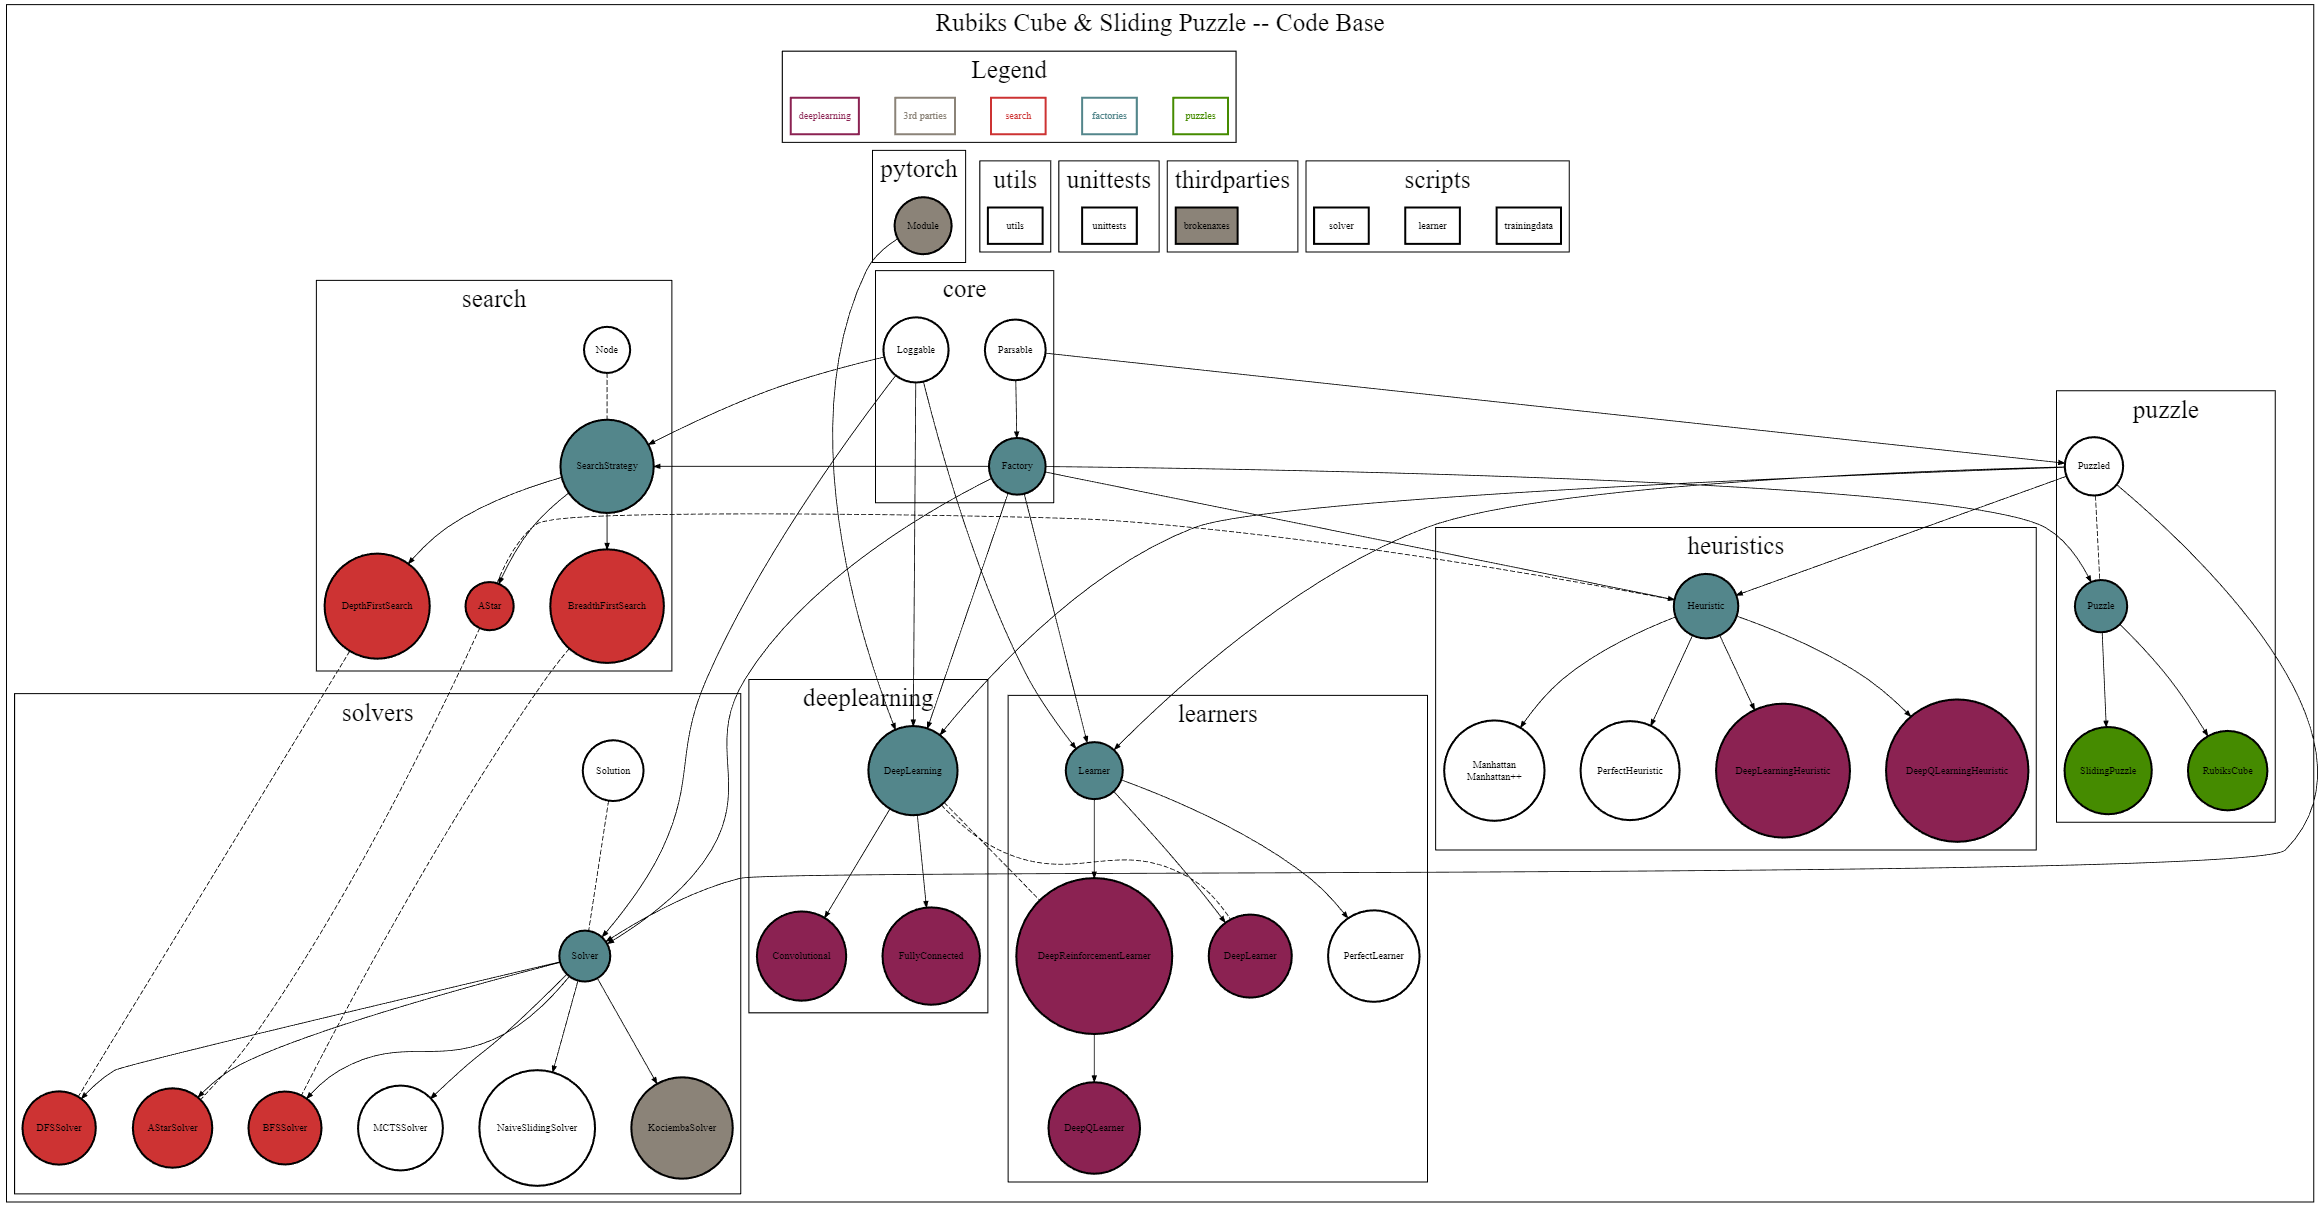
\includegraphics[scale=0.5]{./Figures/codebase}
%\decoRule
\caption[Codebase]{Code base}
\label{fig:Codebase}
\end{figure}
\end{landscape}


Let me describe what each submodule does:

\subsection{rubiks.core}
This submodule contains bases classes that make the code base easier to use, debug, and extend. It contains three base classes:
\begin{itemize}
\item Loggable: a wrapper around Python's logger which automatically picks up classes' names at init and format things (dict, series and dataframes in particular) in a nicer way.
\item Parsable: a wrapper around ArgumentParser, which allows to construct objects in the project from command line, to define dependencies between object's configurations and to help a bit with typing of configs. The end result is that you can pretty much pass **kw\_args everywhere and it just works.
\item Factory: a typical factory pattern. Concrete factories can just define what widget they produce and the factory will help construct them from **kw\_args (or command line, since Factory inherits from Parsable)
\end{itemize}

\subsection{rubiks.puzzle}
This submodule contains:
\begin{itemize}
\item Puzzle: a Factory of puzzles. It defines states and actions in the abstract, and provides useful functions to apply moves, shuffle, generate training sets, tell if a state is the goal, etc. Puzzle can manufacture the two following types of puzzles:
\item SlidingPuzzle. Implements the states and moves of the sliding puzzle.
\item RubiksCube. Implements the states and moves of the Rubik's cube.
\end{itemize}

\subsection{rubiks.heuristics}
This module contains base class Heuristic, also a Factory (the supported widges are Manhattan, specific to the sliding puzzle, discussed in more details in \ref{S33}, )

\subsection{rubiks.search}

\subsection{rubiks.deeplearning}

\subsection{rubiks.learners}

\subsection{rubiks.solvers}


%-----------------------------------
%	SECTION 2
%-----------------------------------
\section{Running An Example}

blabla


%-----------------------------------
%	SECTION 3
%-----------------------------------
\section{DL Training}

blabla
%-----------------------------------
%	SECTION 4
%-----------------------------------
\section{DRL Training}

blabla

%-----------------------------------
%	SECTION 5
%-----------------------------------

\section{Solvers Comparison}

blabla]